\documentclass[a4paper,12pt]{article}

% Pacchetti necessari
\usepackage[utf8]{inputenc}
\usepackage[T1]{fontenc}
\usepackage{graphicx}
\usepackage[italian]{babel}
\usepackage{geometry}
\usepackage{amsmath} 
\usepackage{float}
\usepackage{eso-pic} % Per aggiungere il logo come sfondo
\usepackage{transparent} % Per gestire la trasparenza
\usepackage[hyperindex, bookmarks=true, colorlinks=true, linkcolor=blue, urlcolor=blue]{hyperref}
\usepackage{subfigure} % per inserire due immagini affiancate o per raggruppare in un unico blocco più immagini


% Margini della pagina
\geometry{a4paper, margin=2.5cm}

% Inserimento logo in bianco e nero con opacità
\newcommand\BackgroundLogo{
    \AddToShipoutPictureBG{
        \AtPageLowerLeft{
            \hspace{-3cm}
            \vspace{-4cm}
            \transparent{0.08}
            
\includegraphics[width=12cm, keepaspectratio]{_assets/logo-universita-bn.png}
        }
    }
}

% Comando per abilitare il logo trasparente
\BackgroundLogo

\begin{document}

% Titolo del documento
\begin{titlepage}
    \centering

    \begin{tabular}{@{}c@{\hspace{0.5cm}}c@{}}
        
        \raisebox{-.5\height}{
\includegraphics[width=4cm]{_assets/logo-dipartimento.png}} \\
    \end{tabular}\\[1cm]
    
    {\LARGE Università degli Studi di Salerno}\\[0.5cm]
    {\Large Dipartimento di Ingegneria dell'Informazione ed Elettrica e Matematica Applicata (DIEM)}\\[2cm]
    {\Huge \textbf{Relazione di progetto}}\\[0.4cm]
    {\Large \textbf{Sviluppo di un modello di regressione lineare su dataset}}\\[1cm]
    {\Large Corso di Statistica Applicata - A.A. 2024/25}\\[2cm]
    \begin{flushright}
        \textbf{Studenti Gruppo 16:}\\[0.2cm]
        Corradomaria Giachetta \\
        Matricola: 0612708054 \\
        Francesco Peluso \\
        Matricola: 0612707469 \\[0.2cm]
        Gerardo Selce \\
        Matricola: 0612707692 \\[0.2cm]
        Anuar Zouhri \\
        Matricola: 0612707505 \\[0.2cm]
        \vspace{1cm}
        \textbf{Docenti:}\\
        Prof. Fabio Postiglione \\ Prof. Paolo Addesso 
    \end{flushright}
    \vfill
    Last update: {\large \today}
\end{titlepage}

% Indice
\tableofcontents
\newpage
\section{Descrizione del dataset fornito}
A completezza del progetto si riporta la descrizione del dataset da analizzare. Il dataset contiene $n=100$ osservazioni, costituite da:

\subsection*{Variabile dipendente}
\textbf{y\_VideoQuality} \quad $\rightarrow$ \quad Qualità percepita del video

Tale indice è immaginato come frutto di una opportuna trasformazione di un punteggio assegnato a un campione di immagini da volontari che compilano un questionario. Esso sarà funzione di diverse caratteristiche proprie dei video, tra cui:

\begin{itemize}
	\item la presenza o meno di rumore;
	\item la presenza o meno di \textit{motion blur};
	\item la nitidezza;
	\item la profondità di campo;
	\item la risoluzione;
	\item le aberrazioni ottiche visibili;
	\item la gamma dinamica;
	\item la fedeltà cromatica.
\end{itemize}

\subsection*{Variabili indipendenti (regressori)}

Sono delle quantità di cui l’operatore ha il controllo (parziale o totale) selezionando:

\begin{itemize}
	\item l’attrezzatura video da utilizzare;
	\item i parametri di ripresa.
\end{itemize}

Rappresentano indici standardizzati:

\begin{itemize}
	\item \texttt{x1\_ISO} \quad $\rightarrow$ \quad ISO (sensibilità del sensore)
	\item \texttt{x2\_FRatio} \quad $\rightarrow$ \quad Rapporto Focale
	\item \texttt{x3\_Time} \quad $\rightarrow$ \quad Tempo di Esposizione (in relazione al frame rate utilizzato)
	\item \texttt{x4\_MP} \quad $\rightarrow$ \quad Megapixel del sensore
	\item \texttt{x5\_CROP} \quad $\rightarrow$ \quad Fattore di Crop
	\item \texttt{x6\_FOCAL} \quad $\rightarrow$ \quad Focale
	\item \texttt{x7\_PixDensity} \quad $\rightarrow$ \quad Densità di pixel
\end{itemize}



\newpage
\section{Analisi delle caratteristiche del dataset}
In questa fase preliminare si illustreranno le principali considerazioni fatte sul dataset fornito.
\subsection{Boxplot dei dati}
Si considerino i seguenti boxplot delle variabili del dataset.
\begin{figure}[h]
	\centering
	\subfigure[Boxplot della variabile dipendente y\_VideoQuality]{
		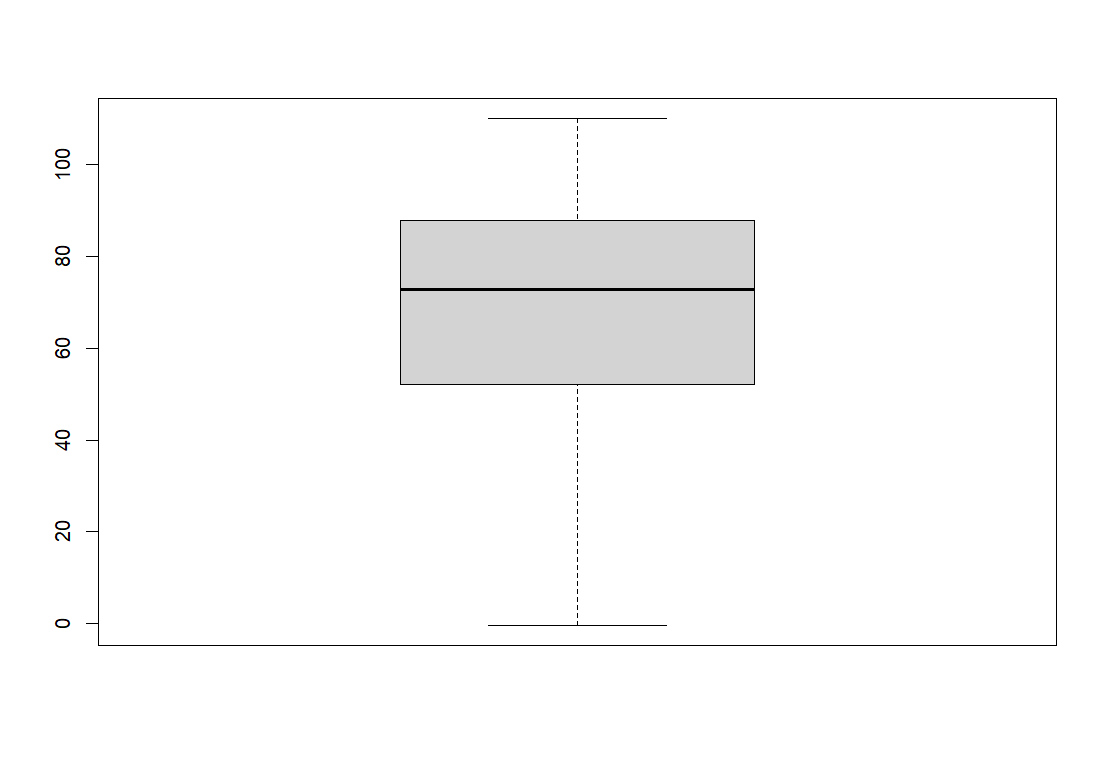
\includegraphics[width=0.65\linewidth]{../graphs/DescriptiveStatisticPlots/boxplot_y_VideoQuality}
		\label{fig:boxplotyvideoquality}
	}
	\subfigure[Boxplot delle variabili indipendenti x\_i]{
		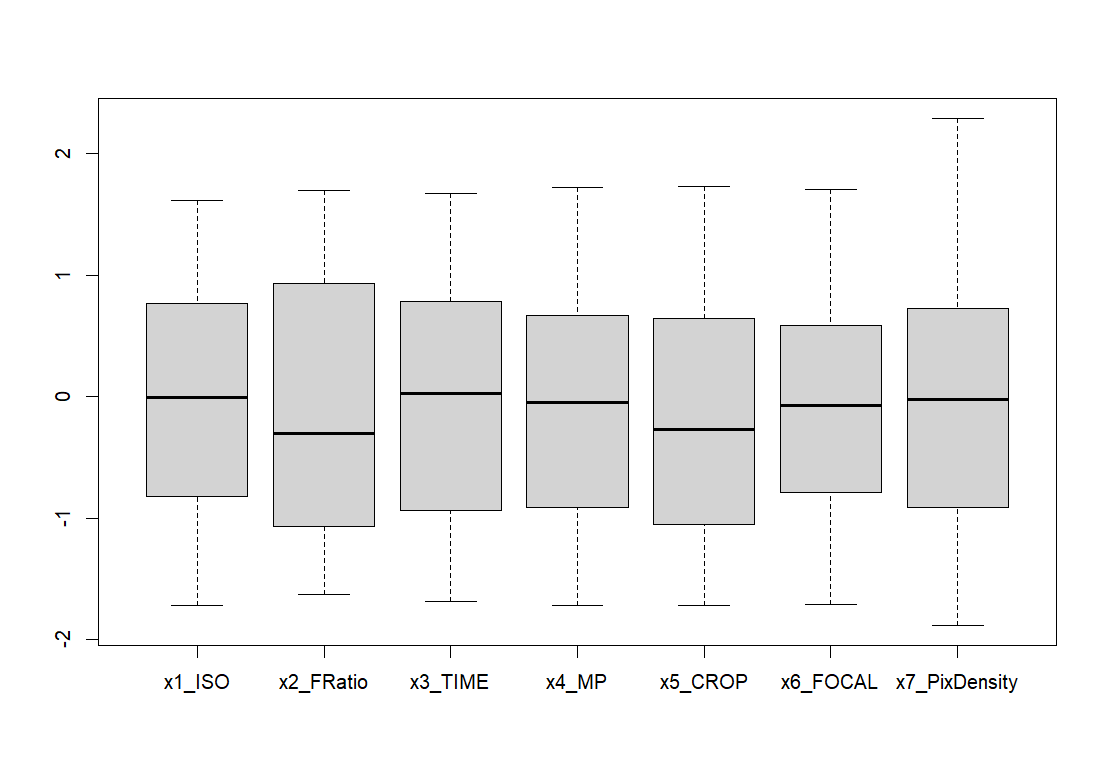
\includegraphics[width=0.65\linewidth]{../graphs/DescriptiveStatisticPlots/boxplot_all_x_i}
		\label{fig:boxplotallxi}
	}
	\caption{Boxplot delle variabili considerate}
\end{figure}

Si osservi innanzitutto che i valori per ciascuna variabile sono tutti contenuti all'interno dell'intervallo interquartile e che quindi non sono presenti outliers. Per quel che riguarda la variabile dipendente y\_VideoQuality si è osservato che il valore della media e della mediana sono simili, infatti valgono rispettivamente  $\text{media}=72.8135, \text{mediana}=68.6081$. Si è osservato inoltre che i valori assunti dalla variabile x7$\_$PixDensity coprono un intervallo maggiore rispetto alle altre variabili indipendenti. 
\subsection{Analisi di normalità}
Anche se non strettamente necessario ai fini del metodo di regressione, si è comunque deciso di verificare se qualcuna delle variabili indipendenti avesse una distribuzione normale.\begin{figure}[h]
	\centering
	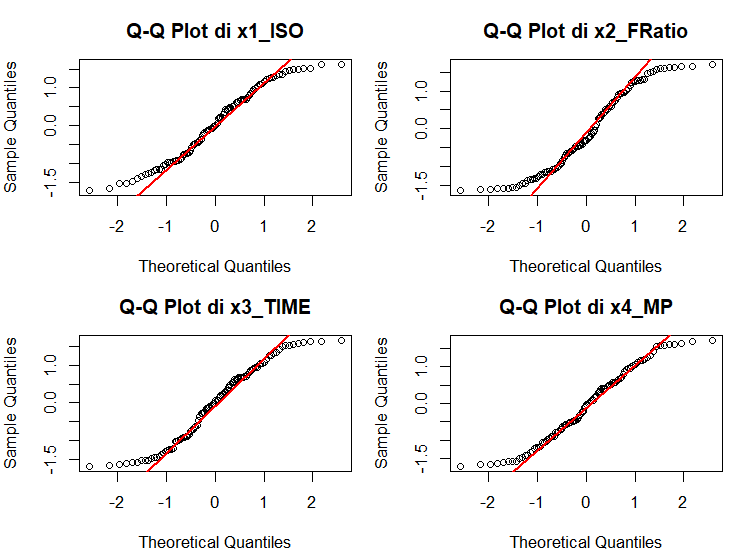
\includegraphics[width=0.9\linewidth]{../graphs/DescriptiveStatisticPlots/qqplot1/qqplot1}
	\caption{}
	\label{fig:qqplot1}
\end{figure}
Tra i diversi qq-plot, si osserva che la variabile x6$\_$Focal sembrerebbe avere una distribuzione normale. Applicando il test di shapiro a questa variabile si ottiene
\begin{align*}
	\text{W} = 0.97, \text{p-value} = 0.02.
\end{align*}
Il valore di p-value ottenuto non si discosta molto da 0.05 e si potrebbe perciò supporre che la variabile sia distribuita come una normale.
\begin{figure}[h]
	\subfigure{
		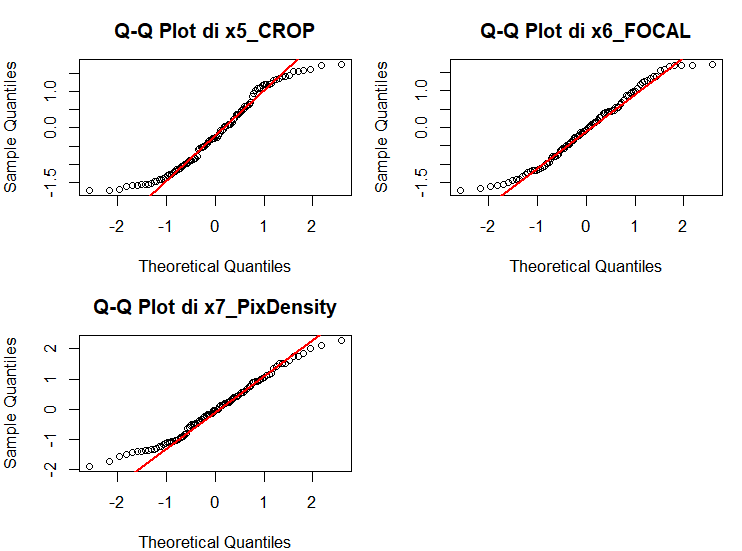
\includegraphics[width=0.9\linewidth]{../graphs/DescriptiveStatisticPlots/qqplot1/qqplot2}
		\label{fig:qqplot2}	
		}
\end{figure}





\newpage
\section{Analisi della dipendenza tra le variabili}


\subsection{Analisi di correlazione}

\begin{figure}[H]
	\centering
	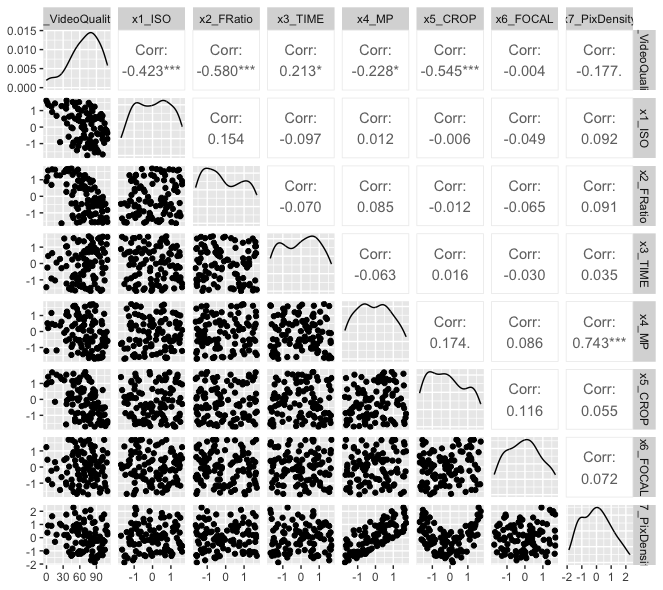
\includegraphics[width=0.90\textwidth]{../graphs/DescriptiveStatisticPlots/ggplot}
	\caption{Scatter plot delle variabili presenti nel dataset.}
\end{figure}

Dalla Figura (3) notiamo, anche dal coefficiente di correlazione, una dipendenza lineare tra le variabili:
\begin{itemize}
	\item \textbf{x4\_MP} e \textbf{x7\_PixDensity}
\end{itemize}
Invece notiamo la presenza di dipendenze non lineari che non vengono descritte dal coefficiente di correlazione. In particolare la notiamo tra le variabili:
\begin{itemize}
	\item \textbf{y\_VideoQuality} e \textbf{x1\_ISO}
	\item \textbf{y\_VideoQuality} e \textbf{x2\_FRatio}
	\item \textbf{y\_VideoQuality} e \textbf{x3\_Time}
	\item \textbf{y\_VideoQuality} e \textbf{x5\_CROP}
	\item \textbf{x5\_CROP} e \textbf{x7\_PixDensity}
\end{itemize}

\subsection{Analisi di regressione}
Le dipendenze tra la variabile y\_VideoQuality e le diverse variabili indipendenti sono state analizzate attraverso una regressione semplice sulle singole variabili indipendenti.
\begin{table}[H]
	\centering
	\begin{tabular}{|c|c|}
		\hline
		\textbf{Variabile indipendente} & \textbf{p-value} \\
		\hline
		x1\_ISO & $1.17e-05$ \\
		\hline
		x2\_FRatio & $2.63e-10$ \\ 
		\hline
		x3\_TIME & $0.0331e$ \\
		\hline
		x4\_MP & $0.0227$ \\
		\hline
		x5\_CROP & $4.39e-09$ \\
		\hline
		x6\_FOCAL & $0.97$ \\
		\hline
		x7\_PixDensity & $0.0775$ \\
		\hline
	\end{tabular}
	\caption{Sono rappresentati i p-value relativi alle regressioni delle singole variabili indipendenti al primo grado.}
	\label{tab:}
\end{table}
Diversamente da quanto ottenuto nell'analisi di correlazione, dalla Tabella (1) risultano rilevanti i regressori x1, x2, x3. La stessa analisi è stata poi effettuata considerando anche i regressori al secondo ordine.

\begin{table}[H]
	\centering
	\begin{tabular}{|c|c|}
		\hline
		\textbf{Variabile indipendente} & \textbf{p-value} \\
		\hline
		x1\_ISO & $2.46e-03$ \\
		\hline
		x2\_FRatio & $1.28e-3$ \\ 
		\hline
		x3\_TIME & $0.3094$ \\
		\hline
		x4\_MP & $0.2899$ \\
		\hline
		x5\_CROP & $0.368$ \\
		\hline
		x6\_FOCAL & $0.770$ \\
		\hline
		x7\_PixDensity & $0.8038$ \\
		\hline
	\end{tabular}
	\caption{Sono rappresentati i p-value relativi alle regressioni delle singole variabili indipendenti al secondo grado.}
	\label{tab:}
\end{table}
Dalla Tabella (2) risulta evidente una dipendenza quadratica della variabile dipendente dai regressori x1, x2.




\end{document}
